% ==============================================================================
%
%                             U S E R   G U I D E
%
% ==============================================================================

% ==============================================================================
%
%                                  S E T U P
%
% ==============================================================================
\chapter{Setup} % <<< -------------------------------------------------------- %
\label{ch:userguide:setup}
% ---------------------------------------------------------------------------- %

Initializing the system and using  the oscilloscope is mostly straightforward,
even for beginners. A few notes on the  initial setup are outlined here to get
the reader started. The next chapter then  presents the general concept of the
user interface.

Getting the system  up and running requires two  basic steps: Initializing the
STEMlab  itself,  and  connecting  to  it  from  a  web  browser  to  run  the
oscilloscope.  Assuming the  STEMlab board at hand has been  delivered with an
SD card  containing the correct Linux  image from this project,  the procedure
for this is as follows:
\begin{enumerate}
    \item
        Insert the SD card coming  with the board (\emph{Note:} Check that the
        SD card has the right side up to make pin contact).
    \item
        Connect the board physically to the network.
    \item
        Connect the board to the power supply.
    \item
        Call    the    board's    IP    address    and    the    right    port
        (eg.    \code{https://10.84.130.54:50090})    in    a    browser    of
        your   preference   (for   best    results   use   Chrome   61.0   and
        above). Figure~\ref{fig:userguide:url} shows  an example  how to
        do this.
    \item  
        A  notice   that  a  popup   menu  has  been  blocked   should  appear
        (Figure~\ref{fig:userguide:popup:warn}). Select   \emph{Always   allow
        popups from  this application}  or similar  and reload  the previously
        called   page. Figure~\ref{fig:userguide:popup:yes}  illustrates   the
        necessary setting.
    \item
        A popup tab should now contain  the scope and automatically connect to
        the  STEMlab's  webserver. Figure~\ref{fig:userguide:running} shows  a
        running scope.
\end{enumerate}

If it  is unknown  whether the  SD card  was delivered  with a  prebuilt image,
it  can  be  assumed  that  it  was  and  the  board  can  be  powered  on. If
the  LED  farthest away  from  the  ports (RJ45,  SD  card,  \ldots )  flashes
orange  with \SI{2}{\Hz},  the SD  card  is fine.   If  the SD  card does  not
contain a  prebuilt image,  Section~\ref{sec:devguide:fpga_toolchain:linux} in
the Developer's Guide explains how one can be acquired or built.

\begin{figure}
    \centering
    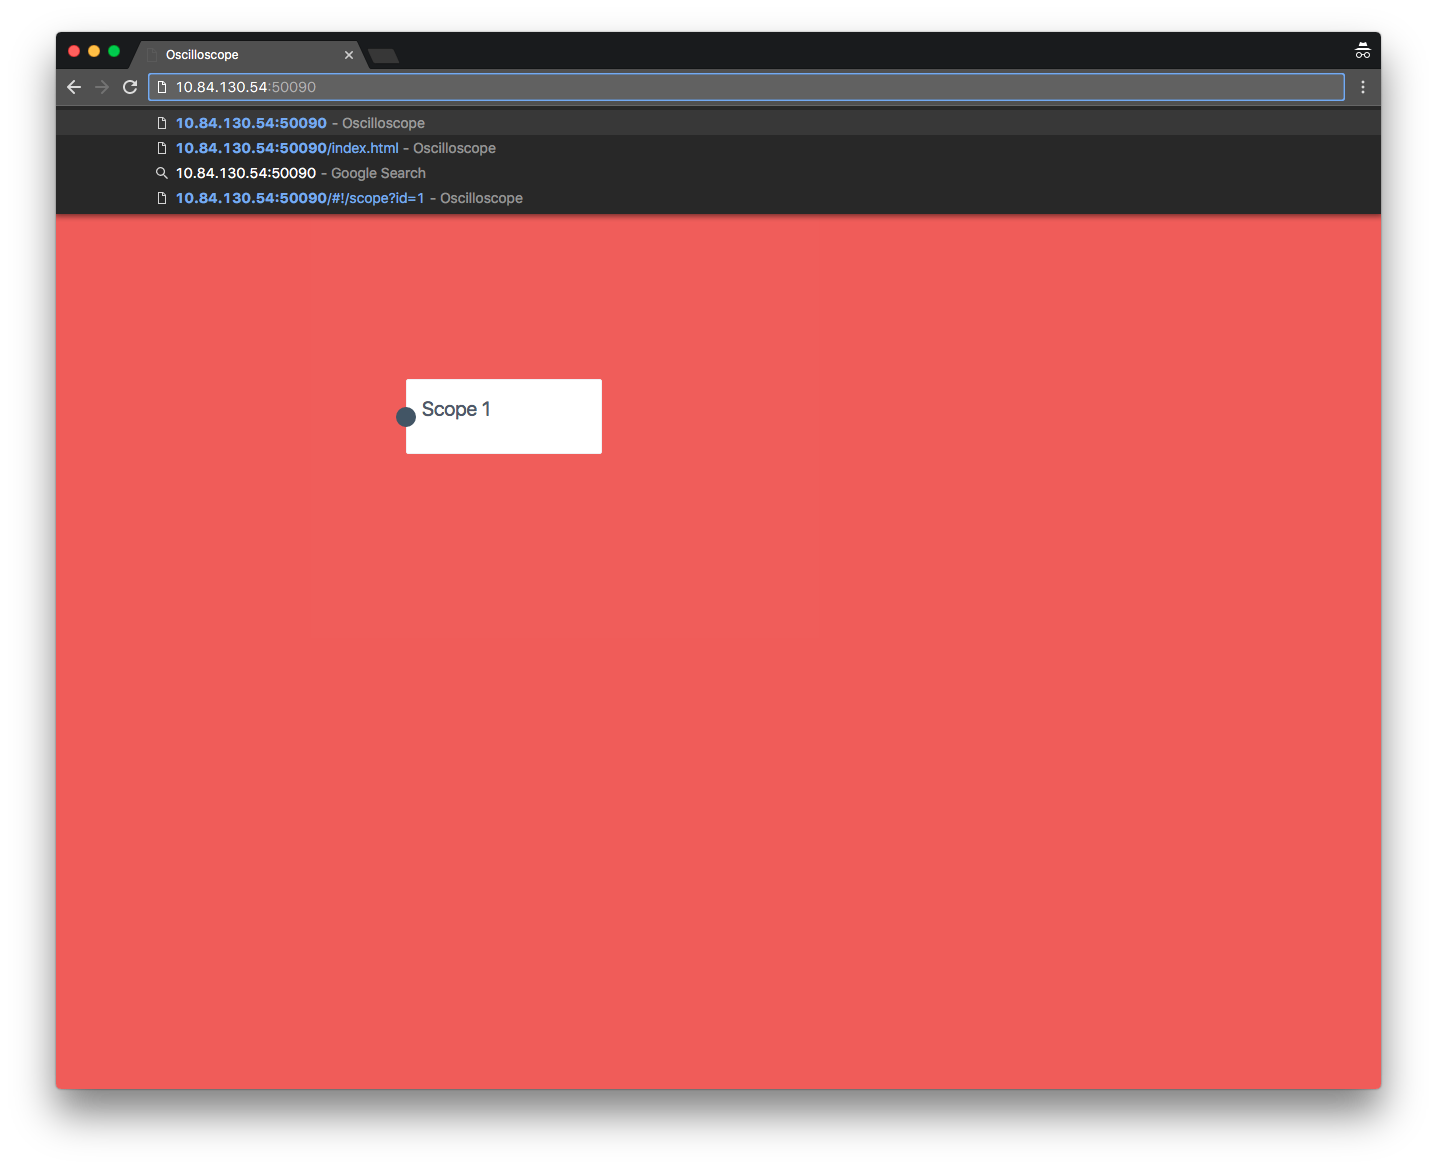
\includegraphics[width=0.75\textwidth]{images/userguide/url}
    \caption[Entering the URL]{%
        Using a browser and the correct URL to run the scope application on
        the STEMlab.
    }
    \label{fig:userguide:url}
\end{figure}

\begin{figure}
    \centering
    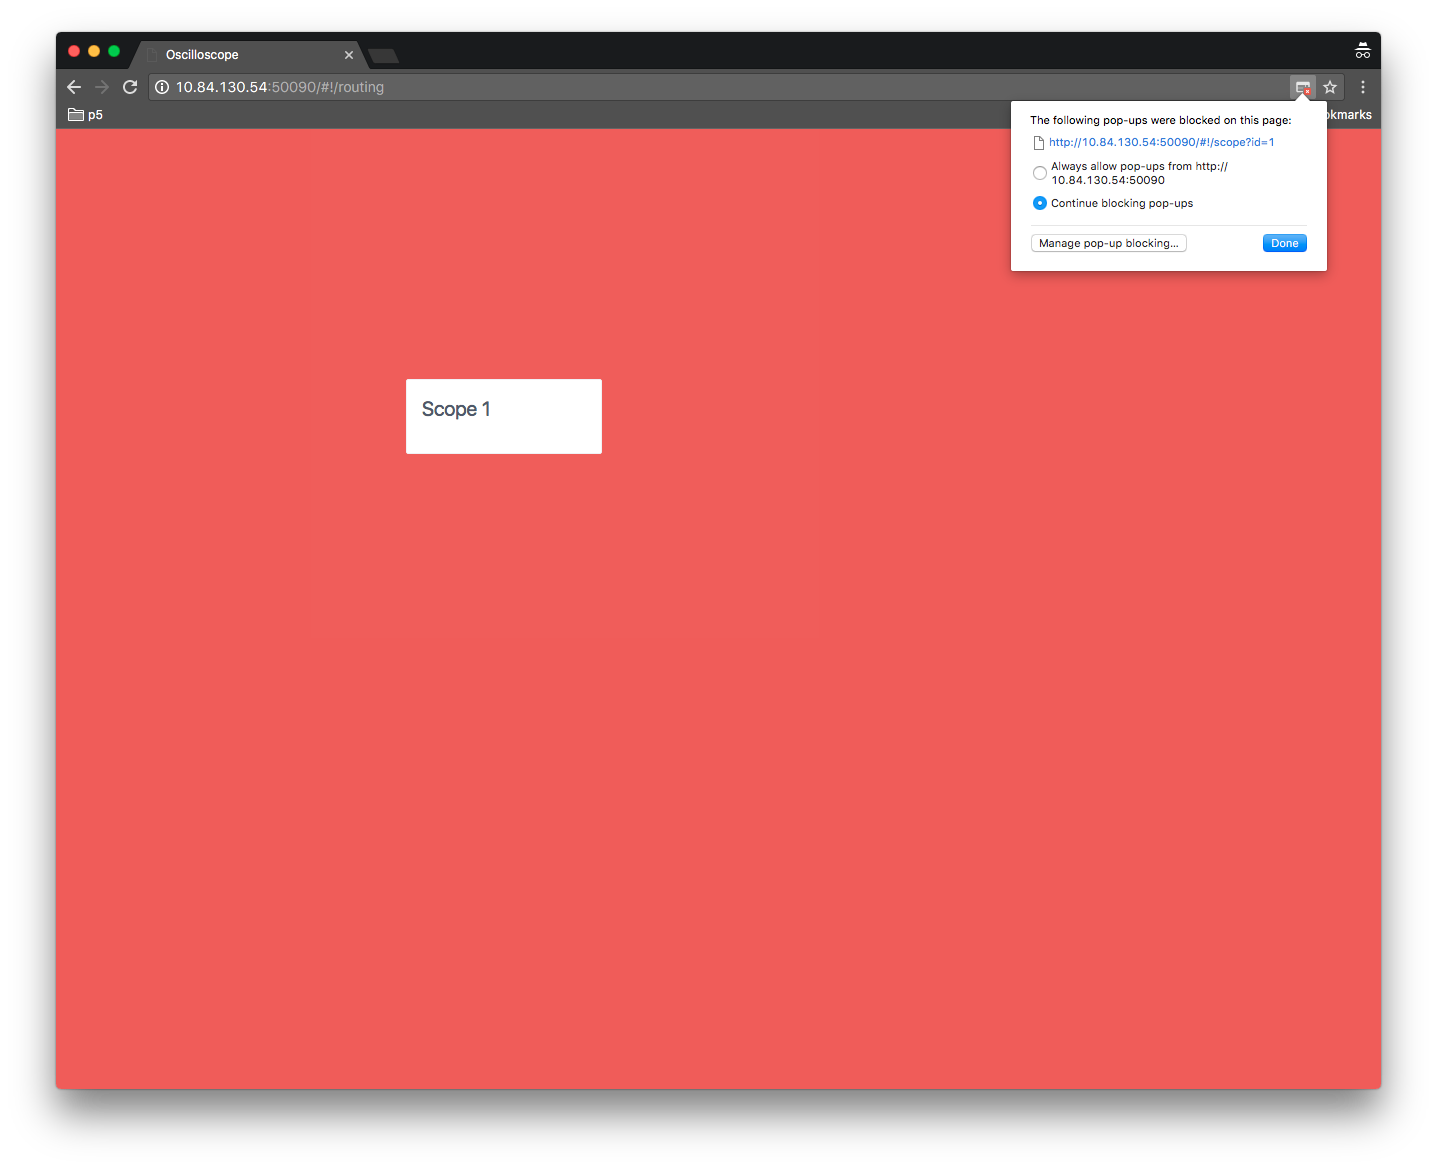
\includegraphics[width=0.75\textwidth]{images/userguide/popup_warn}
    \caption[The popup warn popup]{%
        The browser warns about a popup the site has tried to open.
    }
    \label{fig:userguide:popup:warn}
\end{figure}

\begin{figure}
    \centering
    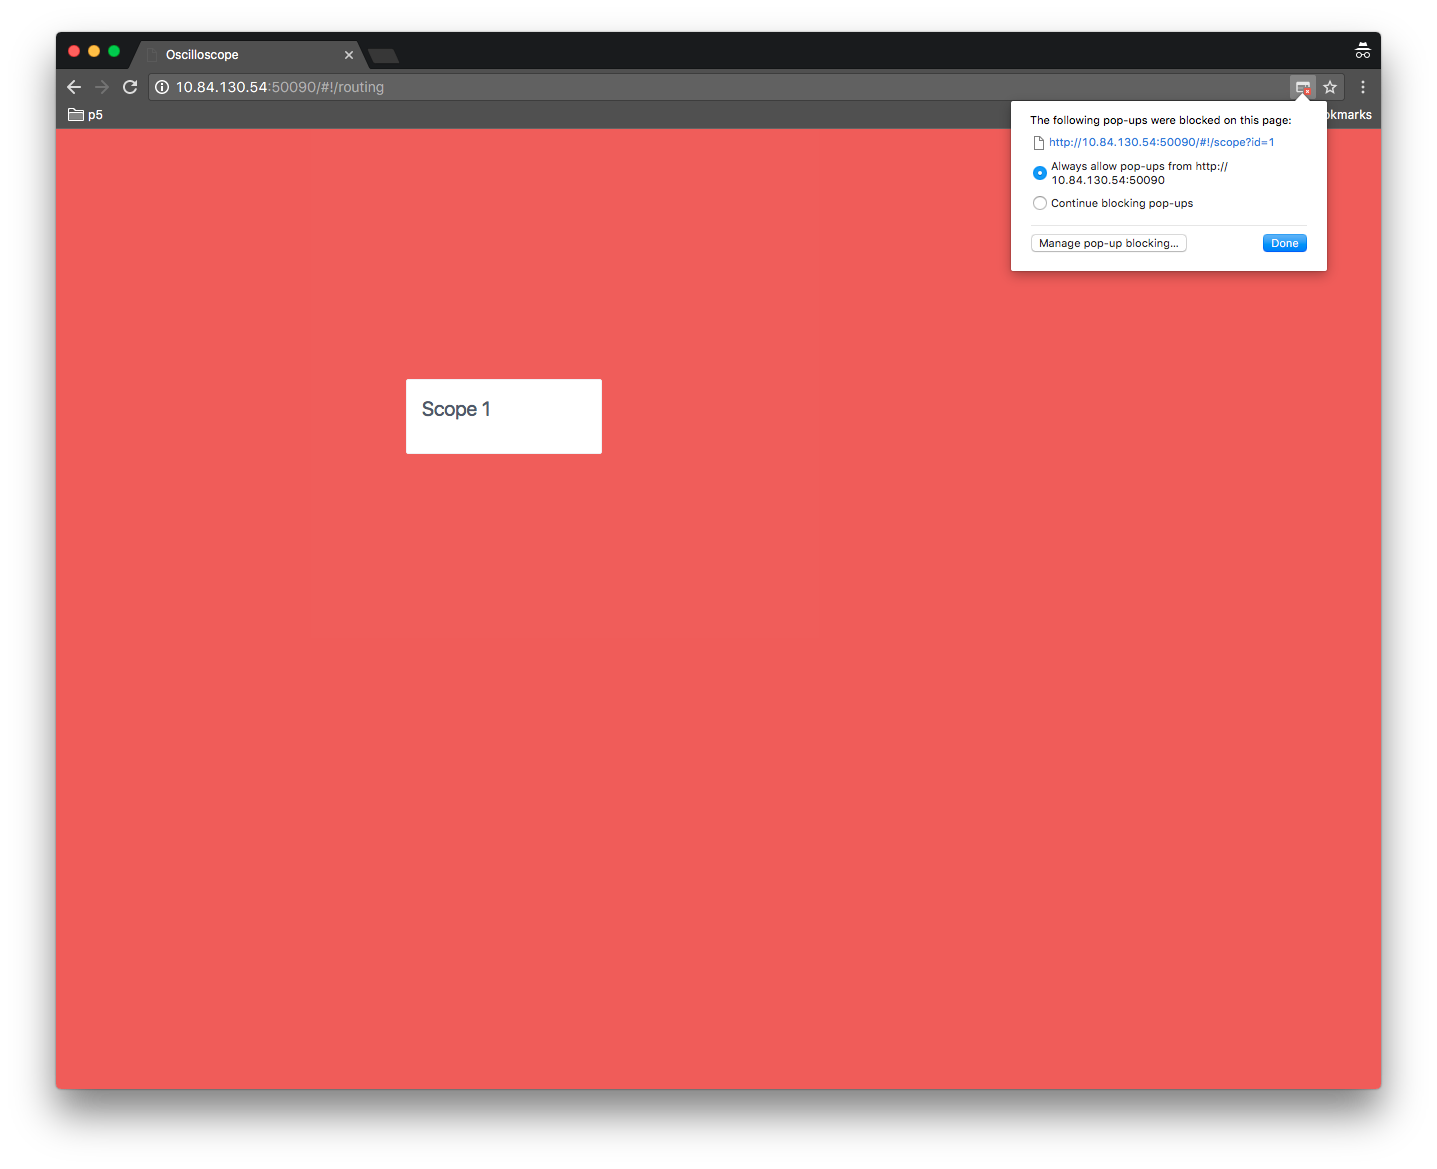
\includegraphics[width=0.75\textwidth]{images/userguide/popup_yes}
    \caption[Accept popups in the future]{%
        Let the browser accept popups in the future.
    }
    \label{fig:userguide:popup:yes}
\end{figure}

\begin{figure}
    \centering
    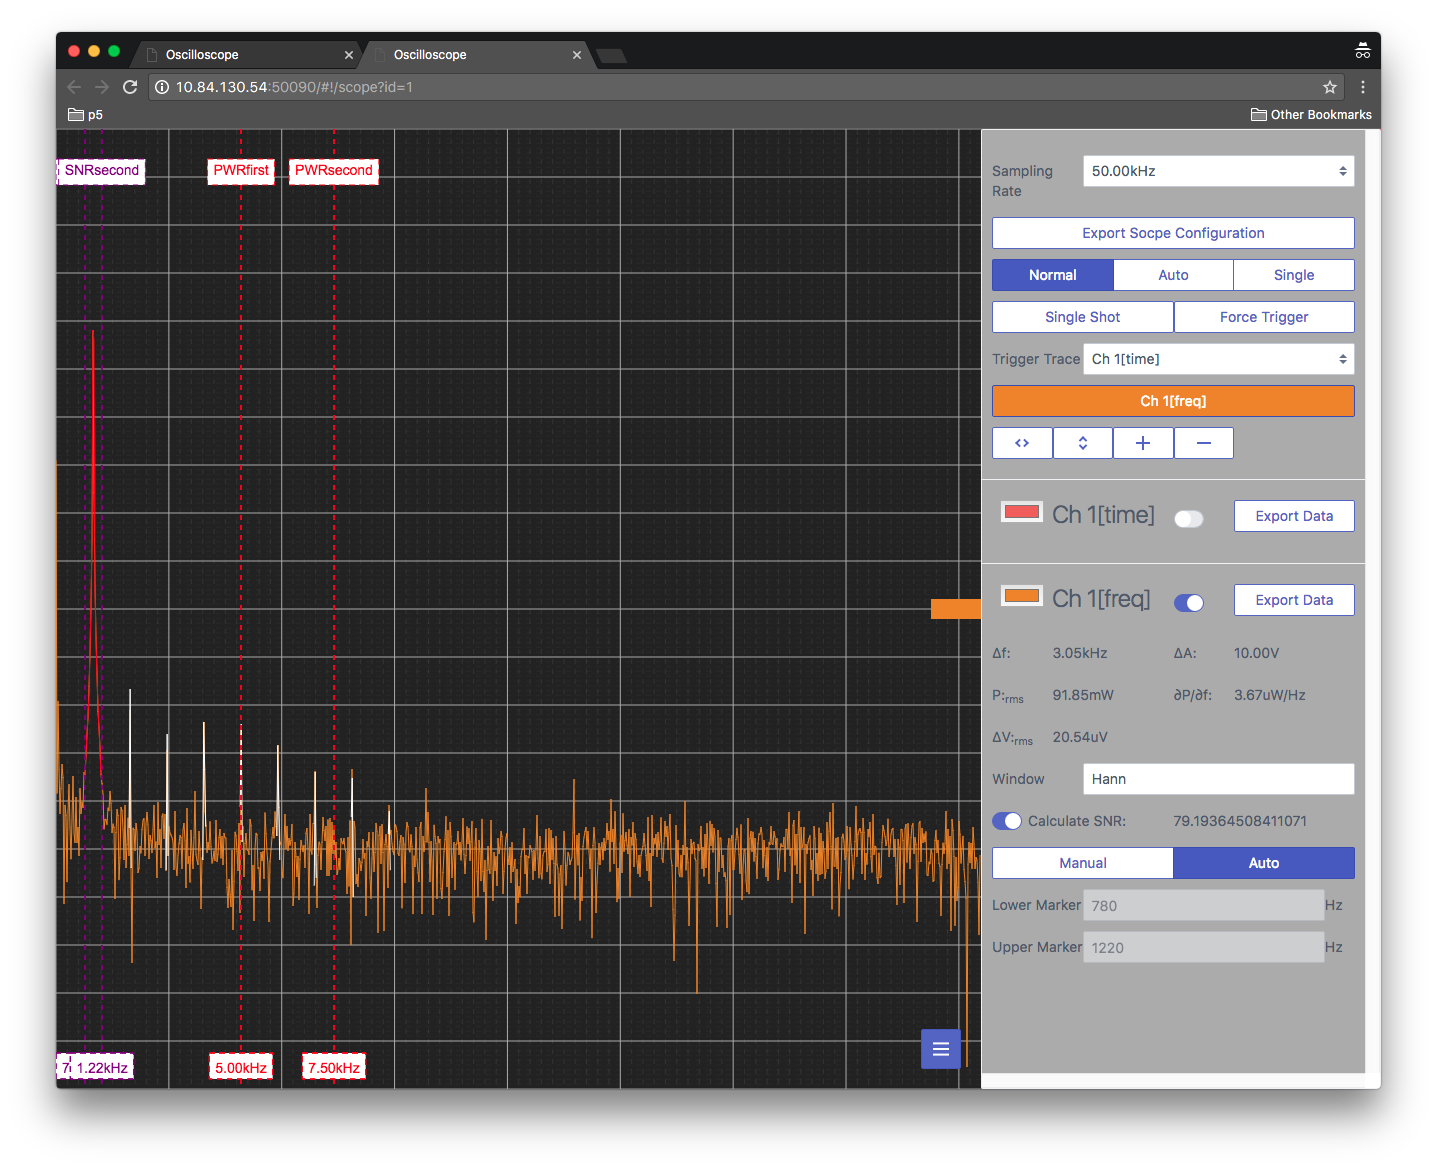
\includegraphics[width=0.75\textwidth]{images/userguide/running}
    \caption[Running the scope]{%
        The running scope after everything has been set up properly.
    }
    \label{fig:userguide:running}
\end{figure}

%>>>
% ==============================================================================
%
%                              O P E R A T I O N
%
% ==============================================================================
\chapter{Operation} % <<< ---------------------------------------------------- %
\label{ch:userguide:operation}
% ---------------------------------------------------------------------------- %

Once the oscilloscope  is running, interaction is done via  its graphical user
interface. Its  most important  features  are summarized  here.   It has  been
designed with high discoverability of its functionality in mind, so a complete
guide on every single  last button and menu is considered  beyond the scope of
this document.

Figure~\ref{fig:userguide:screenshot}  shows a  screenshot  of the  interface.
The UI's most important functions are:
\begin{description}
    \item[Zooming and Panning:]
        To zoom,  use the  vertical and horizontal  scrolling function  of the
        mouse or  trackpad.  To  pan, click  and drag  the signal. If  you are
        dragging a time trace it will automatically move the trigger location.

        The two arrow buttons in the general preference pane resize the signal
        to the visible area.
    \item[Triggering:]
        To set the trigger level, move the drawn trigger level by clicking and
        dragging it  or enter the level  in numbers on the  preference pane of
        the triggering time trace.
    \item[Markers:]
        There are four  markers by default. Two mark the start  and end of the
        area  over which  power  is  integrated and  two  mark  the area  that
        contains the signal for the automatic SNR calculation.

        Markers can be dragged and  moved by clicking and dragging. The number
        at the bottom of each marker shows the frequency it is at.

        The plus button in  the general pref pane adds a  new marker which can
        be used to mark certain frequencies.

        To move the SNR  markers, the SNR mode has to  be set from \emph{auto}
        to \emph{manual} mode in the corresponding FFT trace preference pane.
    \item[Sampling Rate:]
        To configure the  sampling rate, use the drop-down menu  at the top of
        the general preference pane.
    \item[Line Width:]
        To  improve  readability,  some  people  might  like  a  thicker  line
        width. To set the line width, use the  input at the top of the general
        pref pane.
\end{description}

\begin{figure}
    \centering
    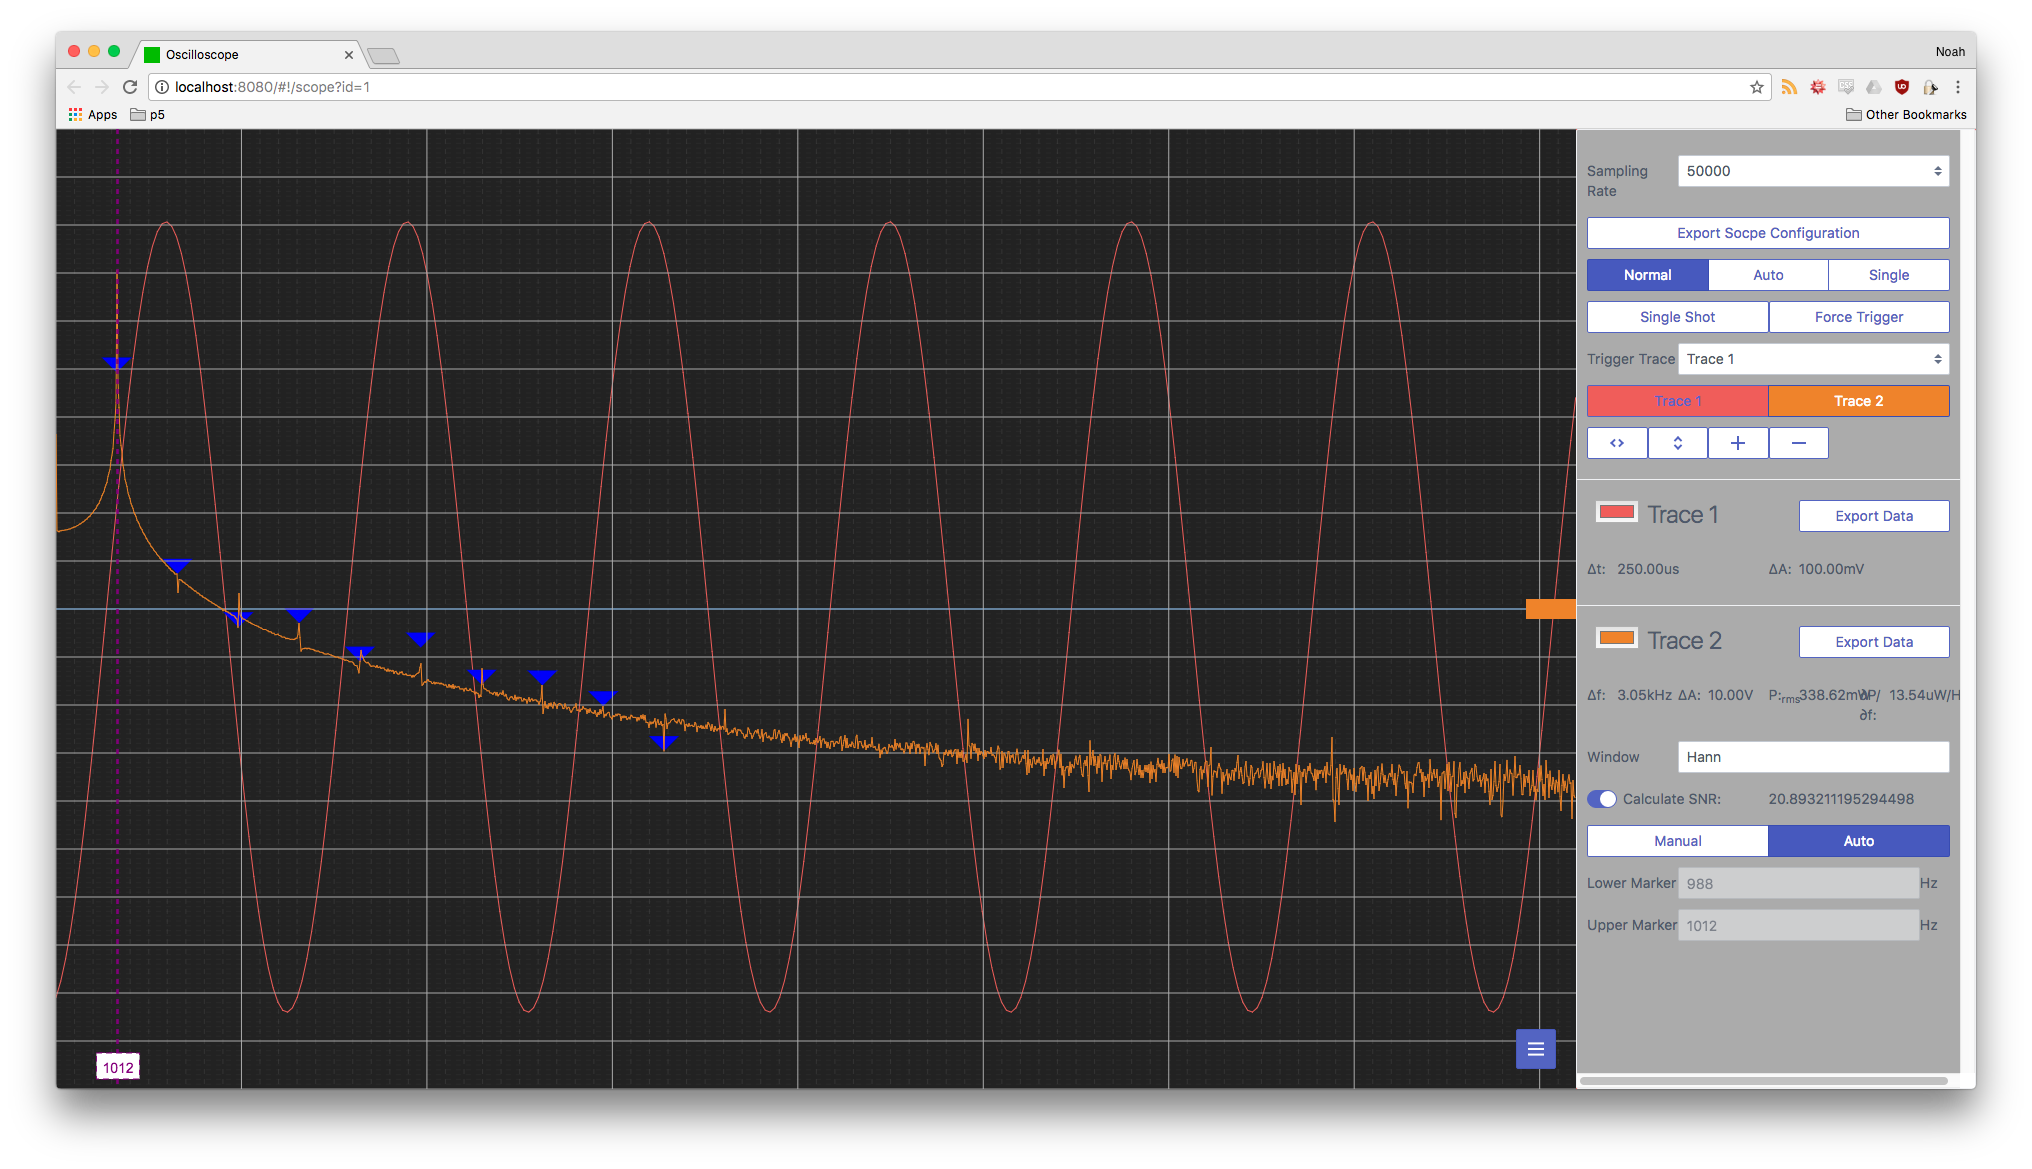
\includegraphics[width=1\textwidth]{images/gui/scope}
    \caption[The Scope Application]{%
        The scope application in its current state, displaying time and FFT data%
    }
    \label{fig:usegruide:screenshot}
\end{figure}

%>>>

%^^A vim: foldenable foldcolumn=4 foldmethod=marker foldmarker=<<<,>>>
